\titre{}
\theme{}
\auteur{Nathan Scheinmann}
\niveau{}
\source{}
\type{serie}
\piments{1}
\pts{}
\annee{2526}

\contenu{
  \qrcode{https://coopmaths.fr/alea/?uuid=b8946&id=1mF1-3&uuid=0e1c6&id=1mF1-17&lang=fr-CH&v=eleve&es=1211001}
	\tcblower
\begin{center}
	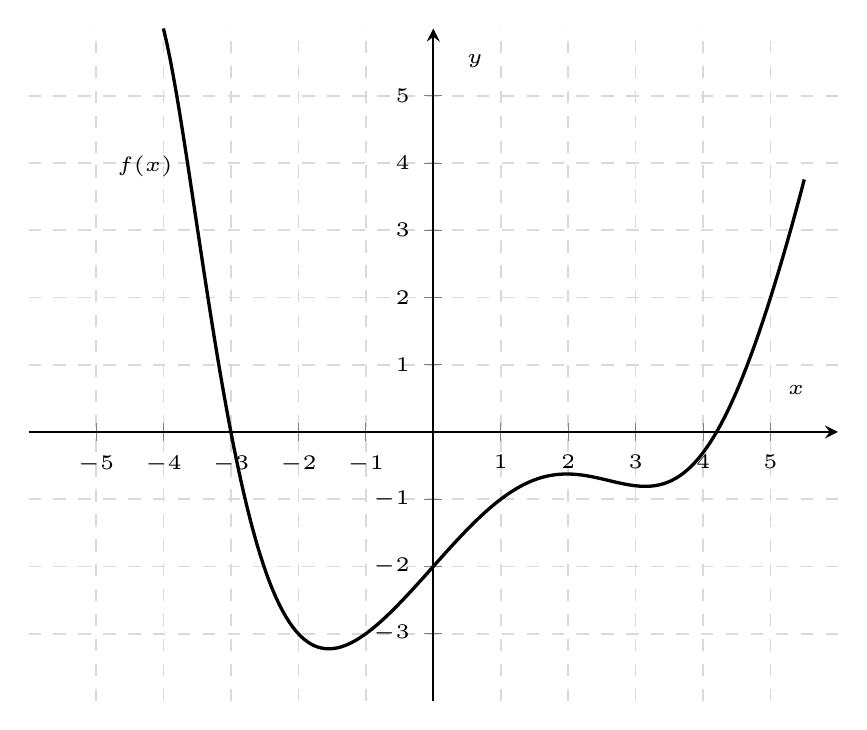
\begin{tikzpicture}[scale=1.5]
  \begin{axis}[
    axis lines=middle,
    xlabel={$x$}, ylabel={$y$},
    every axis x label/.style={at={(ticklabel* cs:0.92)}, anchor=west, yshift=10pt},
    every axis y label/.style={at={(ticklabel* cs:0.92)}, anchor=south, xshift=10pt},
    xmin=-6,   xmax=6,
    ymin=-4,   ymax=6,
    xtick={-5,-4,-3,-2,-1,0,1,2,3,4,5},
    ytick={-3,-2,-1,0,1,2,3,4,5},
    grid=both,
    grid style={dashed,gray!30},
    tick label style={font=\tiny},
    xlabel style={font=\tiny},
    ylabel style={font=\tiny}
  ]
    % branche pour x > 9
    \addplot[domain=-4:5.5, samples=200, thick]
      {-2 + 1.12406*x - 0.0055405*x^2 - 0.120957*x^3 + 0.00248144*x^4 - 0.00311538*x^5 + 0.003193*x^6 + 0.00000448489*x^7 - 0.000133948 *x^8 + 0.0000122393*x^9
}
      node[left,pos=0.1, font=\tiny] {$f(x)$};
  \end{axis}
\end{tikzpicture}
\end{center}

Estimer en observant le graphe~:
\begin{tasks}
  \task la valeur de $f(0)$;
  \task la valeur de $f(-2)$;
  \task les valeurs de $x$ pour lesquelles $f(x)=0$;
  \task la préimage de $2$;
  \task la valeur de $a$ dans l'équation $f(x)=a$ sachant que cette équation ne possède qu'une;
  seule solution. Qu'elle est cette solution ?
  \task les valeurs de $x$ tels que $f(x)=x$;
  \task les valeurs de $x$ tels que $f(x)=-x$.
\end{tasks}


}
\correction{
	\tcblower

}
